\clearpage

\section{Opaque with 1+1 protection}\label{ILP_Opaque_Protection}

\subsection{Model description}

Once more, firstly in order to be able to apply the ILP model we have to take into account the physical and logical topologies allowed by this mode of transport and the type of survivability. Again based in section \ref{opaque} we can conclude that both topologies are the same and the following figures can be confirmed.\\

\begin{figure}[h!]
\centering
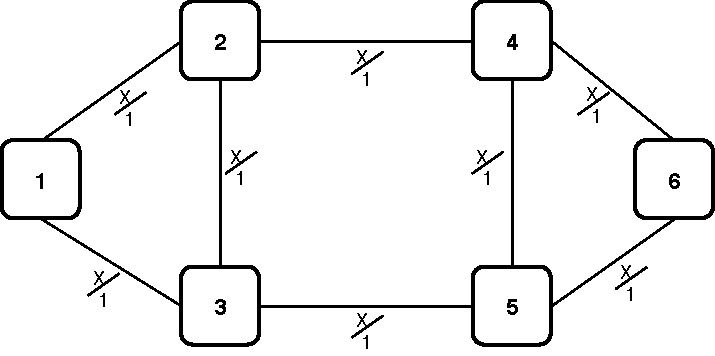
\includegraphics[width=10cm]{sdf/ilp/opaque_protection/figures/allowed_physical_topology}
\caption{Opaque with 1+1 protection: allowed physical topology. The allowed physical topology is defined by the duct and sites in the field. It is assumed that each duct supports up to 1 bidirectional transmission system and each site supports up to 1 node.}
\label{allowed_physical_protectionlow}
\end{figure}

\vspace{13pt}
\begin{figure}[h!]
\centering
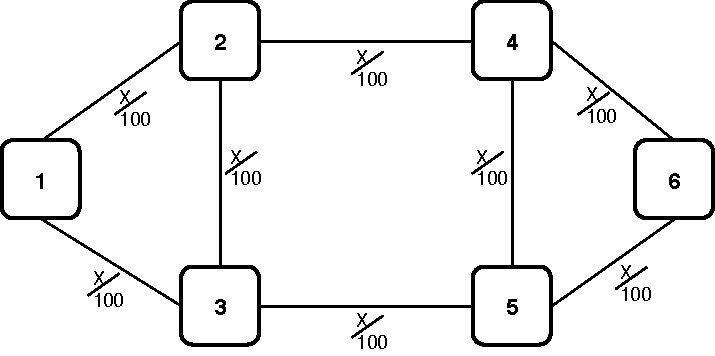
\includegraphics[width=10cm]{sdf/ilp/opaque_protection/figures/allowed_optical_topology}
\caption{Opaque with 1+1 protection: allowed optical topology. The allowed optical topology is defined by the transport mode. It is assumed that each transmission system supports up to 100 optical channels.}
\label{allowed_optical_protectionlow}
\end{figure}

Now taking this into account and based on the specific constraints of the opaque mode with 1+1 protection it is possible to define the ILP model \cite{tesevasco}.\\
\newpage
The objective function, to be minimized, is the expression \ref{Capex}, i.e.,

\begin{equation*}
  minimize \qquad \Big\{ \quad C_C \quad \Big\}
\end{equation*}

$subject$ $to$
\begin{equation}
\sum_{j=1\textbackslash \{o\}}^{N} fb_{ij}^{od} = 2  \qquad \qquad \qquad \qquad \qquad \qquad \qquad \qquad \qquad
\forall(o,d) : o < d, \forall i: i = o
\label{ILPOpaque1}
\end{equation}
\noindent
Constraint \ref{ILPOpaque1} is equal to the constraint \ref{ILPOpaque1_CAPEX} assuming that Z = 2.

\begin{equation}
\sum_{j=1\textbackslash \{o\}}^{N} fb_{ij}^{od} = \sum_{j=1\textbackslash \{d\}}^{N} f_{ji}^{od}   \qquad \qquad \qquad \qquad \qquad \qquad
\forall(o,d) : o < d, \forall i: i \neq o,d
\label{ILPOpaque2}
\end{equation}
\noindent
Constraint \ref{ILPOpaque2} is equal to the constraint \ref{ILPOpaque2_CAPEX}

\begin{equation}
\sum_{j=1\textbackslash \{d\}}^{N} fb_{ji}^{od} = 2  \qquad \qquad \qquad \qquad \qquad \qquad \qquad \qquad \qquad
\forall(o,d) : o < d, \forall i: i = d
\label{ILPOpaque3}
\end{equation}
\noindent
Constraint \ref{ILPOpaque3} is equal to the constraint \ref{ILPOpaque3_CAPEX} assuming that Z = 2.

\begin{equation}
\sum_{o=1}^{N} \sum_{d=o+1}^{N} \left(fb_{ij}^{od} + fb_{ji}^{od}\right) \sum_{c=1}^{C} (B\left(c\right) D_{odc})\leq \tau W_{ij} G_{ij} \qquad \qquad \qquad \qquad
\forall(i,j) : i < j
\label{ILPOpaque4}
\end{equation}
\noindent
The constraint \ref{ILPOpaque4} is considered the grooming constraint and is equal to the constraint \ref{ILPOpaque4_Surv} referred to in the case without survivability.

\begin{equation}
W_{ij} \leq K_{ij} L_{ij} \qquad \qquad \qquad \qquad \qquad \qquad \qquad \qquad \qquad \qquad \qquad \qquad \forall(i,j) : i < j
\label{ILPOpaque5}
\end{equation}
\noindent
Constraint \ref{ILPOpaque5} refers to the capacity of optical channels where they must be less or equal than the maximum number. For any situation, the maximum number of optical channels per transmission system is 100, that is, $K_{ij}$ = 100.

\begin{equation}
fb_{ij}^{od} , fb_{ji}^{od} , L_{ij} \in \{0,1\} \qquad \qquad \qquad \qquad \qquad \qquad \qquad
\forall(i,j) : i < j, \forall(o,d) : o < d
\label{ILPOpaque6}
\end{equation}
\noindent
The number of flows per demand in this case can be zero if there are no traffic demands or one if considering working or protection traffic, in relation to the use of the link, can be zero if it is not being used or one if is being used.
\newpage
\begin{equation}
W_{ij} \in \mathbb{N}  \qquad \qquad \qquad \qquad \qquad \qquad \qquad \qquad \qquad \qquad \qquad \qquad \qquad
\forall(i,j) : i < j\label{ILPOpaque7}
\end{equation}
\noindent
The last constraint is just needed to ensure the number of optical channels is a positive integer value.\\


\subsection{Result description}

As described in the subsection of network traffic \ref{Reference_Network_Traffic}, we have three values of network traffic so we have to obtain three different CAPEX.
The value of the CAPEX of the network will be calculated based on the costs of the equipment present in the table \ref{table_cost_ilp}.\\

\textbf{Low Traffic Scenario:}\\

In a first phase, we will show the resulting physical and optical topology. These topologies are based on the allowed topologies referred to in the model description and also taking into account the logical topology for all ODU's mentioned in the section \ref{low_scenario}.\\

\begin{figure}[h!]
\centering
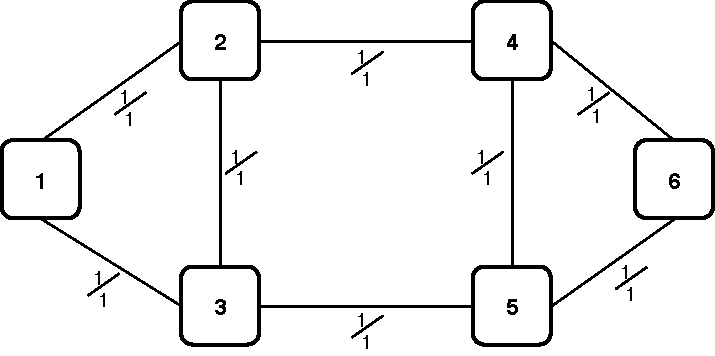
\includegraphics[width=11cm]{sdf/ilp/opaque_protection/figures/physical_topology}
\caption{Opaque with 1+1 protection in low scenario: physical topology after dimensioning.}
\label{physical_protectionlow}
\end{figure}
\newpage
\begin{figure}[h!]
\centering
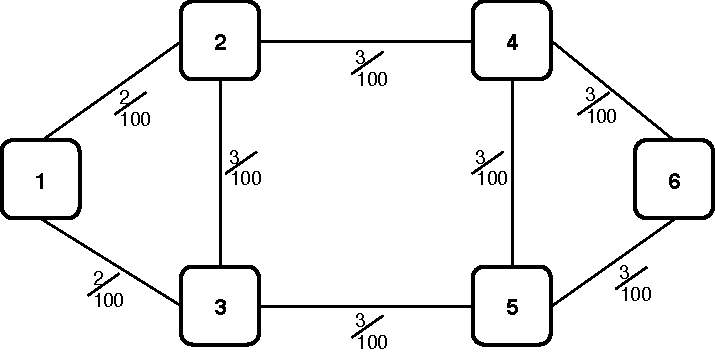
\includegraphics[width=11cm]{sdf/ilp/opaque_protection/figures/optical_topology_low}
\caption{Opaque with 1+1 protection in low scenario: optical topology after dimensioning.}
\label{optical_protectionlow}
\end{figure}

In table \ref{link_opaque_protec_ref_low} we can see the number of optical channels calculated using \ref{Capex_Link} and \ref{ILPOpaque_CAPEX} and the number of amplifiers for each link calculated using \ref{Capex_amplifiers}.

\begin{table}[h!]
\centering
\begin{tabular}{|| c | c | c ||}
 \hline
 \multicolumn{3}{|| c ||}{Information regarding links} \\
 \hline
 \hline
 Bidirectional Link & Optical Channels & Amplifiers\\
 \hline
 Node 1 <-> Node 2 & 2 & 4 \\
 Node 1 <-> Node 3 & 2 & 6 \\
 Node 2 <-> Node 3 & 3 & 0 \\
 Node 2 <-> Node 4 & 3 & 6 \\
 Node 3 <-> Node 5 & 3 & 8 \\
 Node 4 <-> Node 5 & 3 & 1 \\
 Node 4 <-> Node 6 & 3 & 7 \\
 Node 5 <-> Node 6 & 3 & 3 \\
 \hline
\end{tabular}
\caption{Table with information regarding links for opaque mode with 1+1 protection in low scenario.}
\label{link_opaque_protec_ref_low}
\end{table}

In table \ref{node_opaque_protec_ref_low} we can see the resulting nodal degree at the physical layer, calculated based on the number of connections that the node in question performs, the number of line ports calculated using \ref{EXC_pexc1_opaque} and the number of tributary ports calculated using \ref{EXC_pexc2_opaque} for each node.

\begin{table}[h!]
\centering
\begin{tabular}{|| c | c | c | c ||}
 \hline
 \multicolumn{4}{|| c ||}{Information regarding nodes} \\
 \hline
 \hline
 Node & Resulting Nodal Degree & Line Ports & Tributary Ports\\
 \hline
 1 & 2 & 4 & 29 \\
 2 & 3 & 8 & 23 \\
 3 & 3 & 8 & 18 \\
 4 & 3 & 9 & 20 \\
 5 & 3 & 9 & 24 \\
 6 & 2 & 6 & 22 \\
\hline
\end{tabular}
\caption{Table with information regarding nodes for opaque mode with 1+1 protection in low scenario.}
\label{node_opaque_protec_ref_low}
\end{table}
\newpage
Through the information obtained previously on the nodes we can now create tables with detailed information about each node. In each table mentioned below we can see how many ports are connected to a given node and its bit rate and how many ports are assigned to each different bit rate.

\begin{table}[h!]
\centering
\begin{tabular}{|| c | c | c ||}
 \hline
 \multicolumn{3}{|| c ||}{Detailed description of Node 1} \\
 \hline
 \hline
  & Number of tributary ports & Bit rate \\ \hline
\multirow{3}{*}{29 tributary ports} & 13 & ODU0 \\
 & 13 & ODU1 \\
 & 3 & ODU2 \\
 \hline
 \hline
  & Node<--Optical Channels-->Node & Bit rate \\
 \hline
 \multirow{2}{*}{4 line ports} & 1  <---- 2 ---->  2 & \multirow{2}{*}{100 Gbits/s} \\
 & 1  <---- 2 ---->  3 & \\
\hline
\end{tabular}
\caption{Opaque with 1+1 protection in low scenario: detailed description of node 1. The number of demands is distributed to the various destination nodes, this distribution can be observed in section \ref{low_scenario}.}
\end{table}

\begin{table}[h!]
\centering
\begin{tabular}{|| c | c | c ||}
 \hline
 \multicolumn{3}{|| c ||}{Detailed description of Node 2} \\
 \hline
 \hline
  & Number of total demands & Bit rate \\ \hline
\multirow{5}{*}{23 tributary ports} & 11 & ODU0 \\
 & 7 & ODU1 \\
 & 2 & ODU2 \\
 & 2 & ODU3 \\
 & 1 & ODU4 \\
 \hline
 \hline
  & Node<--Optical Channels-->Node & Bit rate \\ \hline
 \multirow{3}{*}{8 line ports} & 2  <---- 2 ---->  1 & \multirow{3}{*}{100 Gbits/s} \\
 & 2  <---- 3 ---->  3 & \\
 & 2  <---- 3 ---->  4 & \\
\hline
\end{tabular}
\caption{Opaque with 1+1 protection in low scenario: detailed description of node 2. The number of demands is distributed to the various destination nodes, this distribution can be observed in section \ref{low_scenario}.}
\end{table}

\begin{table}[h!]
\centering
\begin{tabular}{|| c | c | c ||}
 \hline
 \multicolumn{3}{|| c ||}{Detailed description of Node 3} \\
 \hline
 \hline
  & Number of total demands & Bit rate \\ \hline
\multirow{4}{*}{18 tributary ports} & 7 & ODU0 \\
 & 6 & ODU1\\
 & 3 & ODU2\\
 & 2 & ODU3\\
 \hline
 \hline
   & Node<--Optical Channels-->Node & Bit rate \\ \hline
 \multirow{3}{*}{8 line ports} & 3  <---- 2 ---->  1 & \multirow{3}{*}{100 Gbits/s}\\
 & 3  <---- 3 ---->  2 & \\
 & 3  <---- 3 ---->  5 & \\
\hline
\end{tabular}
\caption{Opaque with 1+1 protection in low scenario: detailed description of node 3. The number of demands is distributed to the various destination nodes, this distribution can be observed in section \ref{low_scenario}.}
\end{table}
\newpage
\begin{table}[h!]
\centering
\begin{tabular}{|| c | c | c ||}
 \hline
 \multicolumn{3}{|| c ||}{Detailed description of Node 4} \\
 \hline
 \hline
  & Number of total demands & Bit rate \\ \hline
\multirow{3}{*}{20 tributary ports} & 7 & ODU0 \\
 & 10 & ODU1 \\
 & 3 & ODU2 \\
 \hline
 \hline
   & Node<--Optical Channels-->Node & Bit rate \\ \hline
 \multirow{3}{*}{9 line ports} & 4  <---- 3 ---->  2 & \multirow{3}{*}{100 Gbits/s}\\
 & 4  <---- 3 ---->  5 & \\
 & 4  <---- 3 ---->  6 & \\
\hline
\end{tabular}
\caption{Opaque with 1+1 protection in low scenario: detailed description of node 4. The number of demands is distributed to the various destination nodes, this distribution can be observed in section \ref{low_scenario}.}
\end{table}

\begin{table}[h!]
\centering
\begin{tabular}{|| c | c | c ||}
 \hline
 \multicolumn{3}{|| c ||}{Detailed description of Node 5} \\
 \hline
 \hline
  & Number of total demands & Bit rate \\ \hline
\multirow{5}{*}{24 tributary ports} & 14 & ODU0 \\
 & 4 & ODU1 \\
 & 4 & ODU2 \\
 & 1 & ODU3 \\
 & 1 & ODU4 \\
 \hline
 \hline
   & Node<--Optical Channels-->Node & Bit rate \\ \hline
 \multirow{3}{*}{9 line ports} & 5  <---- 3 ---->  2 & \multirow{3}{*}{100 Gbits/s}\\
 & 5  <---- 3 ---->  4 & \\
 & 5  <---- 3 ---->  6 & \\
\hline
\end{tabular}
\caption{Opaque with 1+1 protection in low scenario: detailed description of node 5. The number of demands is distributed to the various destination nodes, this distribution can be observed in section \ref{low_scenario}.}
\end{table}

\begin{table}[h!]
\centering
\begin{tabular}{|| c | c | c ||}
 \hline
 \multicolumn{3}{|| c ||}{Detailed description of Node 6} \\
 \hline
 \hline
  & Number of total demands & Bit rate \\ \hline
\multirow{5}{*}{22 tributary ports} & 8 & ODU0 \\
 & 10 & ODU1 \\
 & 1 & ODU2 \\
 & 1 & ODU3 \\
 & 2 & ODU4 \\
 \hline
 \hline
   & Node<--Optical Channels-->Node & Bit rate \\ \hline
 \multirow{2}{*}{6 line ports} & 6  <---- 3 ---->  4 & \multirow{2}{*}{100 Gbits/s}\\
 & 6  <---- 3 ---->  5 & \\
\hline
\end{tabular}
\caption{Opaque with 1+1 protection in low scenario: detailed description of node 6. The number of demands is distributed to the various destination nodes, this distribution can be observed in section \ref{low_scenario}.}
\end{table}

\newpage
In the next table, we can see all the routing obtained for all nodes. These paths are bidirectional so the path from one node to another is the same path in the opposite direction. In the Links column we can see that there are two paths but it is not possible to distinguish them because we do not know which is protection and which is working.

\begin{table}[h!]
\centering
\begin{tabular}{|| c | c | c | c | c | c | c | c ||}
 \hline
 \multicolumn{8}{|| c ||}{Routing} \\
 \hline
 \hline
 o & d & Links & ODU0 & ODU1 & ODU2 & ODU3 & ODU4\\
 \hline
 \multirow{2}{*}{1} & \multirow{2}{*}{2} & \{(1,2)\} & \multirow{2}{*}{5} & \multirow{2}{*}{2} & \multirow{2}{*}{1} & \multirow{2}{*}{0} & \multirow{2}{*}{0} \\
 & & \{(1,3),(3,2)\} & & & & & \\ \hline
 \multirow{2}{*}{1} & \multirow{2}{*}{3} & \{(1,3)\} & \multirow{2}{*}{1} & \multirow{2}{*}{4} & \multirow{2}{*}{1} & \multirow{2}{*}{0} & \multirow{2}{*}{0}\\
 & & \{(1,2),(2,3)\} & & & & &\\ \hline
 \multirow{2}{*}{1} & \multirow{2}{*}{4} & \{(1,2),(2,4)\} & \multirow{2}{*}{3} & \multirow{2}{*}{2} & \multirow{2}{*}{1} & \multirow{2}{*}{0} & \multirow{2}{*}{0}\\
 & & \{(1,3),(3,5),(5,4)\} & & & & &\\ \hline
 \multirow{2}{*}{1} & \multirow{2}{*}{5} & \{(1,3),(3,5)\} & \multirow{2}{*}{1} & \multirow{2}{*}{0} & \multirow{2}{*}{0} & \multirow{2}{*}{0} & \multirow{2}{*}{0}\\
 & & \{(1,2),(2,4),(4,5)\} & & & & &\\ \hline
 \multirow{2}{*}{1} & \multirow{2}{*}{6} & \{(1,2),(2,4),(4,6)\} & \multirow{2}{*}{3} & \multirow{2}{*}{5} & \multirow{2}{*}{0} & \multirow{2}{*}{0} & \multirow{2}{*}{0}\\
 & & \{(1,3),(3,5),(5,6)\} & & & & &\\ \hline
 \multirow{2}{*}{2} & \multirow{2}{*}{3} & \{(2,3)\} & \multirow{2}{*}{0} & \multirow{2}{*}{0} & \multirow{2}{*}{0} & \multirow{2}{*}{1} & \multirow{2}{*}{0}\\
 & & \{(2,1),(1,3)\} & & & & &\\ \hline
 \multirow{2}{*}{2} & \multirow{2}{*}{4} & \{(2,4)\} & \multirow{2}{*}{1} & \multirow{2}{*}{3} & \multirow{2}{*}{0} & \multirow{2}{*}{0} & \multirow{2}{*}{0}\\
 & & \{(2,3),(3,5),(5,4)\} & & & & &\\ \hline
 \multirow{2}{*}{2} & \multirow{2}{*}{5} & \{(2,3),(3,5)\} & \multirow{2}{*}{5} & \multirow{2}{*}{1} & \multirow{2}{*}{1} & \multirow{2}{*}{0} & \multirow{2}{*}{0}\\
 & & \{(2,4),(4,5)\} & & & & &\\ \hline
 \multirow{2}{*}{2} & \multirow{2}{*}{6} & \{(2,4),(4,6)\} & \multirow{2}{*}{0} & \multirow{2}{*}{1} & \multirow{2}{*}{0} & \multirow{2}{*}{1} & \multirow{2}{*}{1}\\
 & & \{(2,3),(3,5),(5,6)\} & & & & &\\ \hline
 \multirow{2}{*}{3} & \multirow{2}{*}{4} & \{(3,2),(2,4)\} & \multirow{2}{*}{1} & \multirow{2}{*}{1} & \multirow{2}{*}{1} & \multirow{2}{*}{0} & \multirow{2}{*}{0}\\
 & & \{(3,5),(5,4)\} & & & & &\\ \hline
 \multirow{2}{*}{3} & \multirow{2}{*}{5} & \{(3,5)\} & \multirow{2}{*}{4} & \multirow{2}{*}{1} & \multirow{2}{*}{1} & \multirow{2}{*}{1} & \multirow{2}{*}{0}\\
 & & \{(3,1),(1,2),(2,4),(4,5)\} & & & & &\\ \hline
 \multirow{2}{*}{3} & \multirow{2}{*}{6} & \{(3,5),(5,6)\} & \multirow{2}{*}{1} & \multirow{2}{*}{0} & \multirow{2}{*}{0} & \multirow{2}{*}{0} & \multirow{2}{*}{0}\\
 & & \{(3,2),(2,4),(4,6)\} & & & & &\\ \hline
 \multirow{2}{*}{4} & \multirow{2}{*}{5} & \{(4,5)\} & \multirow{2}{*}{1} & \multirow{2}{*}{1} & \multirow{2}{*}{1} & \multirow{2}{*}{0} & \multirow{2}{*}{0}\\
 & & \{(4,6),(6,5)\} & & & & &\\ \hline
 \multirow{2}{*}{4} & \multirow{2}{*}{6} & \{(4,6)\} & \multirow{2}{*}{1} & \multirow{2}{*}{3} & \multirow{2}{*}{0} & \multirow{2}{*}{0} & \multirow{2}{*}{0}\\
 & & \{(4,5),(5,6)\} & & & & &\\ \hline
 \multirow{2}{*}{5} & \multirow{2}{*}{6} & \{(5,6)\} & \multirow{2}{*}{3} & \multirow{2}{*}{1} & \multirow{2}{*}{1} & \multirow{2}{*}{0} & \multirow{2}{*}{1}\\
 & & \{(5,4),(4,6)\} & & & & &\\
 \hline
\end{tabular}
\caption{Opaque with 1+1 protection in low scenario: description of routing. We are assuming that between a pair of nodes all demands follow the same route.}
\label{path_opaque_protec_ref_low}
\end{table}

Finally, in next page, through table \ref{scriptopaque_protec_ref_low} we can see the CAPEX result for this model. This value is obtained using equation \ref{ILPOpaque_CAPEX} and all of the constraints mentioned above.\\
\newpage
\begin{table}[h!]
\centering
\begin{tabular}{|| c | c | c | c | c | c | c ||}
 \hline
 \multicolumn{7}{|| c ||}{CAPEX of the Network} \\
 \hline
 \hline
 \multicolumn{3}{|| c |}{ } & Quantity & Unit Price & Cost & Total \\
 \hline
 \multirow{3}{*}{\makecell{Link \\ Cost}} & \multicolumn{2}{ c |}{OLTs} & 16 & 15 000 \euro & 240 000 \euro & \multirow{3}{*}{22 520 000 \euro} \\ \cline{2-6}
 & \multicolumn{2}{ c |}{100 Gbits/s Transceivers} & 44 & 5 000 \euro/Gbit/s & 22 000 000 \euro & \\ \cline{2-6}
 & \multicolumn{2}{ c |}{Amplifiers} & 70 & 4 000 \euro & 280 000 \euro & \\
 \hline
 \multirow{9}{*}{\makecell{Node \\ Cost}} & \multirow{7}{*}{Electrical} & EXCs & 6 & 10 000 \euro & 60 000 \euro & \multirow{9}{*}{4 462 590 \euro} \\ \cline{3-6}
 & & ODU0 Ports & 60 & 10 \euro/port & 600 \euro & \\ \cline{3-6}
 & & ODU1 Ports & 50 & 15 \euro/port & 750 \euro & \\ \cline{3-6}
 & & ODU2 Ports & 16 & 30 \euro/port & 480 \euro & \\ \cline{3-6}
 & & ODU3 Ports & 6 & 60 \euro/port & 360 \euro & \\ \cline{3-6}
 & & ODU4 Ports & 4 & 100 \euro/port & 400 \euro & \\ \cline{3-6}
 & & Line Ports & 44 & 100 000 \euro/port & 4 400 000 \euro & \\ \cline{2-6}
 & \multirow{2}{*}{Optical} & OXCs & 0 & 20 000 \euro & 0 \euro & \\ \cline{3-6}
 & & Ports & 0 & 2 500 \euro/porto & 0 \euro & \\
 \hline
 \multicolumn{6}{|| c |}{Total Network Cost} & 26 982 590 \euro \\
\hline
\end{tabular}
\caption{Opaque with 1+1 protection in low scenario: detailed description of CAPEX for this scenario.}
\label{scriptopaque_protec_ref_low}
\end{table}


\textbf{Medium Traffic Scenario:}\\

In a first phase, we will show the resulting physical and optical topology. These topologies are based on the allowed topologies referred to in the model description and also taking into account the logical topology for all ODU's mentioned in the section \ref{medium_traffic_scenario}.\\

\begin{figure}[h!]
\centering
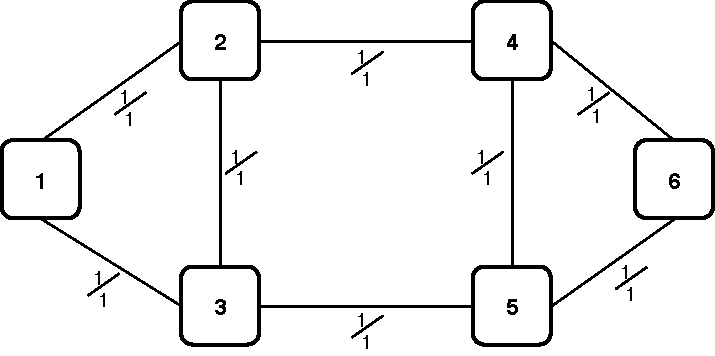
\includegraphics[width=11cm]{sdf/ilp/opaque_protection/figures/physical_topology}
\caption{Opaque with 1+1 protection in medium scenario: physical topology after dimensioning.}
\label{physical_protectionmedium}
\end{figure}
\newpage
\begin{figure}[h!]
\centering
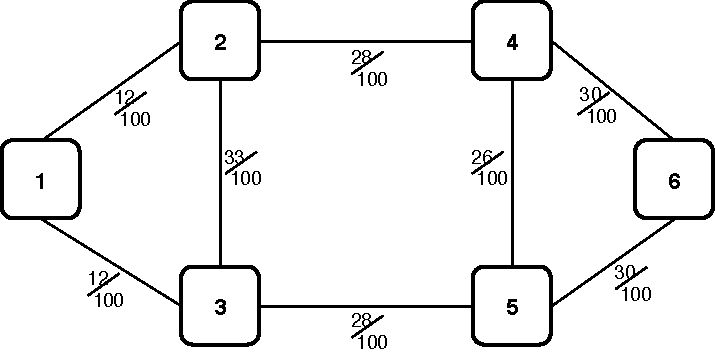
\includegraphics[width=11cm]{sdf/ilp/opaque_protection/figures/optical_topology_medium}
\caption{Opaque with 1+1 protection in medium scenario: optical topology after dimensioning.}
\label{optical_protectionmedium}
\end{figure}

Through table \ref{link_opaque_protec_ref_medium} we can see the number of optical channels calculated using \ref{Capex_Link} and \ref{ILPOpaque_CAPEX} and the number of amplifiers for each link calculated using \ref{Capex_amplifiers}.

\begin{table}[h!]
\centering
\begin{tabular}{|| c | c | c ||}
 \hline
 \multicolumn{3}{|| c ||}{Information regarding links} \\
 \hline
 \hline
 Bidirectional Link & Optical Channels & Amplifiers\\
 \hline
 Node 1 <-> Node 2 & 12 & 4 \\
 Node 1 <-> Node 3 & 12 & 6 \\
 Node 2 <-> Node 3 & 33 & 0 \\
 Node 2 <-> Node 4 & 28 & 6 \\
 Node 3 <-> Node 5 & 28 & 8 \\
 Node 4 <-> Node 5 & 26 & 1 \\
 Node 4 <-> Node 6 & 30 & 7 \\
 Node 5 <-> Node 6 & 30 & 3 \\
 \hline
\end{tabular}
\caption{Table with information regarding links for opaque mode with 1+1 protection in medium scenario.}
\label{link_opaque_protec_ref_medium}
\end{table}

We can see the resulting nodal degree at the physical layer, calculated based on the number of connections that the node in question performs, the number of line ports calculated using \ref{EXC_pexc1_opaque} and the number of tributary ports calculated using \ref{EXC_pexc2_opaque} for each node in table \ref{node_opaque_protec_ref_medium}.

\begin{table}[h!]
\centering
\begin{tabular}{|| c | c | c | c ||}
 \hline
 \multicolumn{4}{|| c ||}{Information regarding nodes} \\
 \hline
 \hline
 Node & Connections & Line Ports & Tributary Ports\\
 \hline
 1 & 2 & 24 & 290 \\
 2 & 3 & 73 & 230 \\
 3 & 3 & 73 & 180 \\
 4 & 3 & 84 & 200 \\
 5 & 3 & 84 & 240 \\
 6 & 2 & 60 & 220 \\
\hline
\end{tabular}
\caption{Table with information regarding nodes for opaque mode with 1+1 protection in medium scenario.}
\label{node_opaque_protec_ref_medium}
\end{table}

\newpage
Once more through the information obtained previously on the nodes we can now create tables with detailed information about each node. In each table mentioned below we can see how many ports are connected to a given node and its bit rate and how many ports are assigned to each different bit rate.

\begin{table}[h!]
\centering
\begin{tabular}{|| c | c | c ||}
 \hline
 \multicolumn{3}{|| c ||}{Detailed description of Node 1} \\
 \hline
 \hline
  & Number of total demands & bit rate \\ \hline
\multirow{3}{*}{290 tributary ports} & 130 & ODU0 \\
 & 130 & ODU1 \\
 & 30 & ODU2 \\
 \hline
 \hline
  & Node <-- Optical Channels --> Node & bit rate \\ \hline
\multirow{2}{*}{24 line ports} & 1  <---- 12 ---->  2 & \multirow{2}{*}{100 Gbtis/s} \\
 & 1  <---- 12 ---->  3 & \\
\hline
\end{tabular}
\caption{Opaque with 1+1 protection in medium scenario: detailed description of node 1. The number of demands is distributed to the various destination nodes, this distribution can be observed in section \ref{medium_traffic_scenario}.}
\end{table}

\begin{table}[h!]
\centering
\begin{tabular}{|| c | c | c ||}
 \hline
 \multicolumn{3}{|| c ||}{Detailed description of Node 2} \\
 \hline
 \hline
  & Number of total demands & bit rate \\ \hline
\multirow{5}{*}{230 tributary ports} & 110 & ODU0 \\
 & 70 & ODU1 \\
 & 20 & ODU2 \\
 & 20 & ODU3 \\
 & 10 & ODU4 \\
 \hline
 \hline
  & Node <-- Optical Channels --> Node & bit rate \\ \hline
 \multirow{3}{*}{73 line ports} & 2  <---- 12 ---->  1 & \multirow{3}{*}{100 Gbtis/s}\\
 & 2  <---- 33 ---->  3 & \\
 & 2  <---- 28 ---->  4 & \\
\hline
\end{tabular}
\caption{Opaque with 1+1 protection in medium scenario: detailed description of node 2. The number of demands is distributed to the various destination nodes, this distribution can be observed in section \ref{medium_traffic_scenario}.}
\end{table}

\begin{table}[h!]
\centering
\begin{tabular}{|| c | c | c ||}
 \hline
 \multicolumn{3}{|| c ||}{Detailed description of Node 3} \\
 \hline
 \hline
  & Number of total demands & bit rate \\ \hline
\multirow{4}{*}{180 tributary ports} & 70 & ODU0 \\
 & 60 & ODU1\\
 & 30 & ODU2\\
 & 20 & ODU3\\
  & Node <-- Optical Channels --> Node & bit rate \\ \hline
 \multirow{3}{*}{73 line ports} & 3  <---- 12 ---->  1 & \multirow{3}{*}{100 Gbtis/s}\\
 & 3  <---- 33 ---->  2 & \\
 & 3  <---- 28 ---->  5 & \\
\hline
\end{tabular}
\caption{Opaque with 1+1 protection in medium scenario: detailed description of node 3. The number of demands is distributed to the various destination nodes, this distribution can be observed in section \ref{medium_traffic_scenario}.}
\end{table}

\newpage
\begin{table}[h!]
\centering
\begin{tabular}{|| c | c | c ||}
 \hline
 \multicolumn{3}{|| c ||}{Detailed description of Node 4} \\
 \hline
 \hline
  & Number of total demands & bit rate \\ \hline
\multirow{3}{*}{200 tributary ports} & 70 & ODU0 \\
 & 100 & ODU1 \\
 & 30 & ODU2 \\
  & Node <-- Optical Channels --> Node & bit rate \\ \hline
\multirow{3}{*}{84 line ports} & 4  <---- 28 ---->  2 & \multirow{3}{*}{100 Gbtis/s}\\
 & 4  <---- 26 ---->  5 & \\
 & 4  <---- 30 ---->  6 & \\
\hline
\end{tabular}
\caption{Opaque with 1+1 protection in medium scenario: detailed description of node 4. The number of demands is distributed to the various destination nodes, this distribution can be observed in section \ref{medium_traffic_scenario}.}
\end{table}

\begin{table}[h!]
\centering
\begin{tabular}{|| c | c | c ||}
 \hline
 \multicolumn{3}{|| c ||}{Detailed description of Node 5} \\
 \hline
 \hline
  & Number of total demands & bit rate \\ \hline
\multirow{5}{*}{240 tributary ports} & 140 & ODU0 \\
 & 40 & ODU1 \\
 & 40 & ODU2 \\
 & 10 & ODU3 \\
 & 10 & ODU4 \\
  & Node <-- Optical Channels --> Node & bit rate \\ \hline
 \multirow{3}{*}{84 line ports} & 5  <---- 28 ---->  3 & \multirow{3}{*}{100 Gbtis/s} \\
 & 5  <---- 26 ---->  4 & \\
 & 5  <---- 30 ---->  6 & \\
\hline
\end{tabular}
\caption{Opaque with 1+1 protection in medium scenario: detailed description of node 5. The number of demands is distributed to the various destination nodes, this distribution can be observed in section \ref{medium_traffic_scenario}.}
\end{table}

\begin{table}[h!]
\centering
\begin{tabular}{|| c | c | c ||}
 \hline
 \multicolumn{3}{|| c ||}{Detailed description of Node 6} \\
 \hline
 \hline
  & Number of total demands & bit rate \\ \hline
\multirow{5}{*}{220 tributary ports} & 80 & ODU0 \\
 & 100 & ODU1 \\
 & 10 & ODU2 \\
 & 10 & ODU3 \\
 & 20 & ODU4 \\
  & Node <-- Optical Channels --> Node & bit rate \\ \hline
 \multirow{2}{*}{60 line ports} & 6  <---- 30 ---->  4 & \multirow{2}{*}{100 Gbtis/s} \\
 & 6  <---- 30 ---->  5 & \\
\hline
\end{tabular}
\caption{Opaque with 1+1 protection in medium scenario: detailed description of node 6. The number of demands is distributed to the various destination nodes, this distribution can be observed in section \ref{medium_traffic_scenario}.}
\end{table}

\newpage
Now let's focus on the routing information. These paths are bidirectional so the path from one node to another is the same path in the opposite direction. In table \ref{path_opaque_protec_ref_medium} we can see all the routing obtained for all nodes. In the Links column we can see that there are two paths but it is not possible to distinguish them because we do not know which is protection and which is working.\\

\begin{table}[h!]
\centering
\begin{tabular}{|| c | c | c | c | c | c | c | c ||}
 \hline
 \multicolumn{8}{|| c ||}{Routing} \\
 \hline
 \hline
 o & d & Links & ODU0 & ODU1 & ODU2 & ODU3 & ODU4\\
 \hline
 \multirow{2}{*}{1} & \multirow{2}{*}{2} & \{(1,2)\} & \multirow{2}{*}{50} & \multirow{2}{*}{20} & \multirow{2}{*}{10} & \multirow{2}{*}{0} & \multirow{2}{*}{0} \\
 & & \{(1,3),(3,2)\} & & & & & \\ \hline
 \multirow{2}{*}{1} & \multirow{2}{*}{3} & \{(1,3)\} & \multirow{2}{*}{10} & \multirow{2}{*}{40} & \multirow{2}{*}{10} & \multirow{2}{*}{0} & \multirow{2}{*}{0}\\
 & & \{(1,2),(2,3)\} & & & & &\\ \hline
 \multirow{2}{*}{1} & \multirow{2}{*}{4} & \{(1,2),(2,4)\} & \multirow{2}{*}{30} & \multirow{2}{*}{20} & \multirow{2}{*}{10} & \multirow{2}{*}{0} & \multirow{2}{*}{0}\\
 & & \{(1,3),(3,5),(5,4)\} & & & & &\\ \hline
 \multirow{2}{*}{1} & \multirow{2}{*}{5} & \{(1,3),(3,5)\} & \multirow{2}{*}{10} & \multirow{2}{*}{0} & \multirow{2}{*}{0} & \multirow{2}{*}{0} & \multirow{2}{*}{0}\\
 & & \{(1,2),(2,4),(4,5)\} & & & & &\\ \hline
 \multirow{2}{*}{1} & \multirow{2}{*}{6} & \{(1,2),(2,4),(4,6)\} & \multirow{2}{*}{30} & \multirow{2}{*}{50} & \multirow{2}{*}{0} & \multirow{2}{*}{0} & \multirow{2}{*}{0}\\
 & & \{(1,3),(3,5),(5,6)\} & & & & &\\ \hline
 \multirow{2}{*}{2} & \multirow{2}{*}{3} & \{(2,3)\} & \multirow{2}{*}{0} & \multirow{2}{*}{0} & \multirow{2}{*}{0} & \multirow{2}{*}{10} & \multirow{2}{*}{0}\\
 & & \{(2,1),(1,3)\} & & & & &\\ \hline
 \multirow{2}{*}{2} & \multirow{2}{*}{4} & \{(2,4)\} & \multirow{2}{*}{10} & \multirow{2}{*}{30} & \multirow{2}{*}{0} & \multirow{2}{*}{0} & \multirow{2}{*}{0}\\
 & & \{(2,3),(3,5),(5,4)\} & & & & &\\ \hline
 \multirow{2}{*}{2} & \multirow{2}{*}{5} & \{(2,4),(4,5)\} & \multirow{2}{*}{50} & \multirow{2}{*}{10} & \multirow{2}{*}{10} & \multirow{2}{*}{0} & \multirow{2}{*}{0}\\
 & & \{(2,3),(3,5)\} & & & & &\\ \hline
 \multirow{2}{*}{2} & \multirow{2}{*}{6} & \{(2,4),(4,6)\} & \multirow{2}{*}{0} & \multirow{2}{*}{10} & \multirow{2}{*}{0} & \multirow{2}{*}{10} & \multirow{2}{*}{10}\\
 & & \{(2,3),(3,5),(5,6)\} & & & & &\\ \hline
 \multirow{2}{*}{3} & \multirow{2}{*}{4} & \{(3,2),(2,4)\} & \multirow{2}{*}{10} & \multirow{2}{*}{10} & \multirow{2}{*}{10} & \multirow{2}{*}{0} & \multirow{2}{*}{0}\\
 & & \{(3,5),(5,4)\} & & & & &\\ \hline
 \multirow{2}{*}{3} & \multirow{2}{*}{5} & \{(3,5)\} & \multirow{2}{*}{40} & \multirow{2}{*}{10} & \multirow{2}{*}{10} & \multirow{2}{*}{10} & \multirow{2}{*}{0}\\
 & & \{(3,2),(2,4),(4,5)\} & & & & &\\ \hline
 \multirow{2}{*}{3} & \multirow{2}{*}{6} & \{(3,5),(5,6)\} & \multirow{2}{*}{10} & \multirow{2}{*}{0} & \multirow{2}{*}{0} & \multirow{2}{*}{0} & \multirow{2}{*}{0}\\
 & & \{(3,2),(2,4),(4,6)\} & & & & &\\ \hline
 \multirow{2}{*}{4} & \multirow{2}{*}{5} & \{(4,5)\} & \multirow{2}{*}{10} & \multirow{2}{*}{10} & \multirow{2}{*}{10} & \multirow{2}{*}{0} & \multirow{2}{*}{0}\\
 & & \{(4,6),(6,5)\} & & & & &\\ \hline
 \multirow{2}{*}{4} & \multirow{2}{*}{6} & \{(4,6)\} & \multirow{2}{*}{10} & \multirow{2}{*}{30} & \multirow{2}{*}{0} & \multirow{2}{*}{0} & \multirow{2}{*}{0}\\
 & & \{(4,5),(5,6)\} & & & & &\\ \hline
 \multirow{2}{*}{5} & \multirow{2}{*}{6} & \{(5,6)\} & \multirow{2}{*}{30} & \multirow{2}{*}{10} & \multirow{2}{*}{10} & \multirow{2}{*}{0} & \multirow{2}{*}{10}\\
 & & \{(5,4),(4,6)\} & & & & &\\
 \hline
\end{tabular}
\caption{Opaque with 1+1 protection in medium scenario: table with description of routing. We are assuming that between a pair of nodes all demands follow the same route.}
\label{path_opaque_protec_ref_medium}
\end{table}

Once more in next page, through table \ref{scriptopaque_protec_ref_medium} we can see the CAPEX result for this model. This value is obtained using equation \ref{ILPOpaque_CAPEX} and all of the constraints mentioned above.\\
\newpage
\begin{table}[h!]
\centering
\begin{tabular}{||c|c|c|c|c|c|c||}
 \hline
 \multicolumn{7}{||c||}{CAPEX of the Network} \\
 \hline
 \hline
 \multicolumn{3}{||c|}{}& Quantity & Unit Price & Cost & Total \\
 \hline
 \multirow{3}{*}{\makecell{Link \\ Cost}} & \multicolumn{2}{c|}{OLTs}&16&15 000 \euro&240 000 \euro&\multirow{3}{*}{199 520 000 \euro}\\ \cline{2-6}
 & \multicolumn{2}{c|}{100 Gbits/s Transceivers}&398&5 000 \euro/Gbit/s&199 000 000 \euro&\\ \cline{2-6}
 & \multicolumn{2}{c|}{Amplifiers}&70&4 000 \euro&280 000 \euro&\\
 \hline
 \multirow{9}{*}{\makecell{Node \\ Cost}}&\multirow{7}{*}{Electrical}&EXCs & 6 & 10 000 \euro & 60 000 \euro & \multirow{9}{*}{39 885 900 \euro} \\ \cline{3-6}
 & &ODU0 Ports& 600 & 10 \euro/port & 6 000 \euro & \\ \cline{3-6}
 & &ODU1 Ports& 500 & 15 \euro/port & 7 500 \euro & \\ \cline{3-6}
 & &ODU2 Ports& 160 & 30 \euro/port & 4 800 \euro & \\ \cline{3-6}
 & &ODU3 Ports& 60 & 60 \euro/port & 3 600 \euro & \\ \cline{3-6}
 & &ODU4 Ports& 40 & 100 \euro/port & 4 000 \euro & \\ \cline{3-6}
 & &Line Ports& 398 &100 000 \euro/port&39 800 000 \euro& \\ \cline{2-6}
 & \multirow{2}{*}{Optical} & OXCs & 0 & 20 000 \euro & 0 \euro & \\ \cline{3-6}
 & & Ports & 0 & 2 500 \euro/porto & 0 \euro & \\
 \hline
 \multicolumn{6}{|| c |}{Total Network Cost} & 239 405 900 \euro \\
\hline
\end{tabular}
\caption{Opaque with 1+1 protection in medium scenario: table with detailed description of CAPEX for this scenario.}
\label{scriptopaque_protec_ref_medium}
\end{table}


\textbf{High Traffic Scenario:}\\

In a first phase, we will show the resulting physical and optical topology. These topologies are based on the allowed topologies referred to in the model description and also taking into account the logical topology for all ODU's mentioned in the section \ref{high_traffic_scenario}.\\

\begin{figure}[h!]
\centering
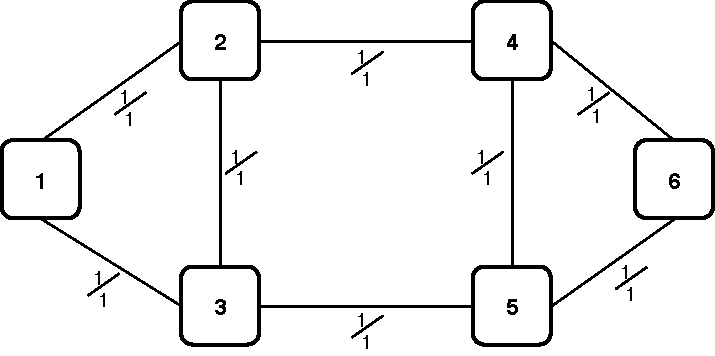
\includegraphics[width=11cm]{sdf/ilp/opaque_protection/figures/physical_topology}
\caption{Opaque with 1+1 protection in high scenario: physical topology after dimensioning.}
\label{physical_protectionhigh}
\end{figure}

\newpage
\begin{figure}[h!]
\centering
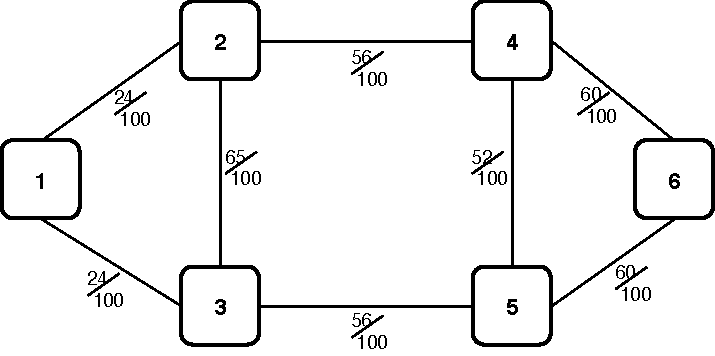
\includegraphics[width=11cm]{sdf/ilp/opaque_protection/figures/optical_topology_high}
\caption{Opaque with 1+1 protection in high scenario: optical topology after dimensioning.}
\label{optical_protectionhigh}
\end{figure}

In table \ref{link_opaque_protec_ref_high} we can see the number of optical channels calculated using \ref{Capex_Link} and \ref{Capex} and the number of amplifiers for each link calculated using \ref{amplifiers}.

\begin{table}[h!]
\centering
\begin{tabular}{|| c | c | c ||}
 \hline
 \multicolumn{3}{|| c ||}{Information regarding links} \\
 \hline
 \hline
 Bidirectional Link & Optical Channels & Amplifiers\\
 \hline
 Node 1 <-> Node 2 & 24 & 4 \\
 Node 1 <-> Node 3 & 24 & 6 \\
 Node 2 <-> Node 3 & 65 & 0 \\
 Node 2 <-> Node 4 & 56 & 6 \\
 Node 3 <-> Node 5 & 56 & 8 \\
 Node 4 <-> Node 5 & 52 & 1 \\
 Node 4 <-> Node 6 & 60 & 7 \\
 Node 5 <-> Node 6 & 60 & 3 \\
 \hline
\end{tabular}
\caption{Table with information regarding links for opaque mode with 1+1 protection in high scenario.}
\label{link_opaque_protec_ref_high}
\end{table}

In table \ref{node_opaque_protec_ref_high} we can see the resulting nodal degree at the physical layer, calculated based on the number of connections that the node in question performs, the number of line ports calculated using \ref{EXC_pexc1_opaque} and the number of tributary ports calculated using \ref{EXC_pexc2_opaque} for each node.

\begin{table}[h!]
\centering
\begin{tabular}{|| c | c | c | c ||}
 \hline
 \multicolumn{4}{|| c ||}{Information regarding nodes} \\
 \hline
 \hline
 Node & Resulting Nodal Degree & Line Ports & Tributary Ports\\
 \hline
 1 & 2 & 48 & 580 \\
 2 & 3 & 145 & 460 \\
 3 & 3 & 145 & 360 \\
 4 & 3 & 168 & 400 \\
 5 & 3 & 168 & 480 \\
 6 & 2 & 120 & 440 \\
\hline
\end{tabular}
\caption{Table with information regarding nodes for opaque mode with 1+1 protection in high scenario.}
\label{node_opaque_protec_ref_high}
\end{table}

\newpage
Once again, through the information obtained previously on the nodes we can now create tables with detailed information about each node. In each table mentioned below we can see how many ports are connected to a given node and its bit rate and how many ports are assigned to each different bit rate.

\begin{table}[h!]
\centering
\begin{tabular}{|| c | c | c ||}
 \hline
 \multicolumn{3}{|| c ||}{Detailed description of Node 1} \\
 \hline
 \hline
  & Number of total demands & bit rate \\ \hline
\multirow{3}{*}{580 tributary ports} & 260 & ODU0 \\
 & 260 & ODU1 \\
 & 60 & ODU2 \\
  & Node <-- Optical Channels --> Node & bit rate \\ \hline
\multirow{2}{*}{48 line ports} & 1  <---- 24 ---->  2 & \multirow{2}{*}{100 Gbtis/s} \\
 & 1  <---- 24 ---->  3 & \\
\hline
\end{tabular}
\caption{Opaque with 1+1 protection in high scenario: detailed description of node 1. The number of demands is distributed to the various destination nodes, this distribution can be observed in section \ref{high_traffic_scenario}.}
\end{table}

\begin{table}[h!]
\centering
\begin{tabular}{|| c | c | c ||}
 \hline
 \multicolumn{3}{|| c ||}{Detailed description of Node 2} \\
 \hline
 \hline
  & Number of total demands & bit rate \\ \hline
\multirow{5}{*}{460 tributary ports} & 220 & ODU0 \\
 & 140 & ODU1 \\
 & 40 & ODU2 \\
 & 40 & ODU3 \\
 & 20 & ODU4 \\
  & Node <-- Optical Channels --> Node & bit rate \\ \hline
 \multirow{3}{*}{145 line ports} & 2  <---- 24 ---->  1 & \multirow{3}{*}{100 Gbtis/s}\\
 & 2  <---- 65 ---->  3 & \\
 & 2  <---- 56 ---->  4 & \\
\hline
\end{tabular}
\caption{Opaque with 1+1 protection in high scenario: detailed description of node 2. The number of demands is distributed to the various destination nodes, this distribution can be observed in section \ref{high_traffic_scenario}.}
\end{table}

\begin{table}[h!]
\centering
\begin{tabular}{|| c | c | c ||}
 \hline
 \multicolumn{3}{|| c ||}{Detailed description of Node 3} \\
 \hline
 \hline
  & Number of total demands & bit rate \\ \hline
\multirow{4}{*}{360 tributary ports} & 140 & ODU0 \\
 & 120 & ODU1\\
 & 60 & ODU2\\
 & 40 & ODU3\\
  & Node <-- Optical Channels --> Node & bit rate \\ \hline
 \multirow{3}{*}{145 line ports} & 3  <---- 24 ---->  1 & \multirow{3}{*}{100 Gbtis/s}\\
 & 3  <---- 65 ---->  2 & \\
 & 3  <---- 56 ---->  5 & \\
\hline
\end{tabular}
\caption{Opaque with 1+1 protection in high scenario: detailed description of node 3. The number of demands is distributed to the various destination nodes, this distribution can be observed in section \ref{high_traffic_scenario}.}
\end{table}

\newpage
\begin{table}[h!]
\centering
\begin{tabular}{|| c | c | c ||}
 \hline
 \multicolumn{3}{|| c ||}{Detailed description of Node 4} \\
 \hline
 \hline
  & Number of total demands & bit rate \\ \hline
\multirow{3}{*}{400 tributary ports} & 140 & ODU0 \\
 & 200 & ODU1 \\
 & 60 & ODU2 \\
  & Node <-- Optical Channels --> Node & bit rate \\ \hline
\multirow{3}{*}{168 line ports} & 4  <---- 56 ---->  2 & \multirow{3}{*}{100 Gbtis/s}\\
 & 4  <---- 52 ---->  5 & \\
 & 4  <---- 60 ---->  6 & \\
\hline
\end{tabular}
\caption{Opaque with 1+1 protection in high scenario: detailed description of node 4. The number of demands is distributed to the various destination nodes, this distribution can be observed in section \ref{high_traffic_scenario}.}
\end{table}

\begin{table}[h!]
\centering
\begin{tabular}{|| c | c | c ||}
 \hline
 \multicolumn{3}{|| c ||}{Detailed description of Node 5} \\
 \hline
 \hline
  & Number of total demands & bit rate \\ \hline
\multirow{5}{*}{480 tributary ports} & 280 & ODU0 \\
 & 80 & ODU1 \\
 & 80 & ODU2 \\
 & 20 & ODU3 \\
 & 20 & ODU4 \\
  & Node <-- Optical Channels --> Node & bit rate \\ \hline
 \multirow{3}{*}{168 line ports} & 5  <---- 56 ---->  3 & \multirow{3}{*}{100 Gbtis/s} \\
 & 5  <---- 52 ---->  4 & \\
 & 5  <---- 60 ---->  6 & \\
\hline
\end{tabular}
\caption{Opaque with 1+1 protection in high scenario: detailed description of node 5. The number of demands is distributed to the various destination nodes, this distribution can be observed in section \ref{high_traffic_scenario}.}
\end{table}

\begin{table}[h!]
\centering
\begin{tabular}{|| c | c | c ||}
 \hline
 \multicolumn{3}{|| c ||}{Detailed description of Node 6} \\
 \hline
 \hline
  & Number of total demands & bit rate \\ \hline
\multirow{5}{*}{440 tributary ports} & 160 & ODU0 \\
 & 200 & ODU1 \\
 & 20 & ODU2 \\
 & 20 & ODU3 \\
 & 40 & ODU4 \\
  & Node <-- Optical Channels --> Node & bit rate \\ \hline
 \multirow{2}{*}{120 line ports} & 6  <---- 60 ---->  4 & \multirow{2}{*}{100 Gbtis/s} \\
 & 6  <---- 60 ---->  5 & \\
\hline
\end{tabular}
\caption{Opaque with 1+1 protection in high scenario: detailed description of node 6. The number of demands is distributed to the various destination nodes, this distribution can be observed in section \ref{high_traffic_scenario}.}
\end{table}

\newpage
Now through the table \ref{path_opaque_protec_ref_high} we can see all the routing obtained for all nodes. These paths are bidirectional so the path from one node to another is the same path in the opposite direction. In the Links column we can see that there are two paths but it is not possible to distinguish them because we do not know which is protection and which is working.

\begin{table}[h!]
\centering
\begin{tabular}{|| c | c | c | c | c | c | c | c ||}
 \hline
 \multicolumn{8}{|| c ||}{Routing} \\
 \hline
 \hline
 o & d & Links & ODU0 & ODU1 & ODU2 & ODU3 & ODU4\\
 \hline
 \multirow{2}{*}{1} & \multirow{2}{*}{2} & \{(1,2)\} & \multirow{2}{*}{100} & \multirow{2}{*}{40} & \multirow{2}{*}{20} & \multirow{2}{*}{0} & \multirow{2}{*}{0} \\
 & & \{(1,3),(3,2)\} & & & & & \\ \hline
 \multirow{2}{*}{1} & \multirow{2}{*}{3} & \{(1,3)\} & \multirow{2}{*}{20} & \multirow{2}{*}{80} & \multirow{2}{*}{20} & \multirow{2}{*}{0} & \multirow{2}{*}{0}\\
 & & \{(1,2),(2,3)\} & & & & &\\ \hline
 \multirow{2}{*}{1} & \multirow{2}{*}{4} & \{(1,2),(2,4)\} & \multirow{2}{*}{60} & \multirow{2}{*}{40} & \multirow{2}{*}{20} & \multirow{2}{*}{0} & \multirow{2}{*}{0}\\
 & & \{(1,3),(3,5),(5,4)\} & & & & &\\ \hline
 \multirow{2}{*}{1} & \multirow{2}{*}{5} & \{(1,3),(3,5)\} & \multirow{2}{*}{20} & \multirow{2}{*}{0} & \multirow{2}{*}{0} & \multirow{2}{*}{0} & \multirow{2}{*}{0}\\
 & & \{(1,2),(2,4),(4,5)\} & & & & &\\ \hline
 \multirow{2}{*}{1} & \multirow{2}{*}{6} & \{(1,2),(2,4),(4,6)\} & \multirow{2}{*}{60} & \multirow{2}{*}{100} & \multirow{2}{*}{0} & \multirow{2}{*}{0} & \multirow{2}{*}{0}\\
 & & \{(1,3),(3,5),(5,6)\} & & & & &\\ \hline
 \multirow{2}{*}{2} & \multirow{2}{*}{3} & \{(2,3)\} & \multirow{2}{*}{0} & \multirow{2}{*}{0} & \multirow{2}{*}{0} & \multirow{2}{*}{20} & \multirow{2}{*}{0}\\
 & & \{(2,1),(1,3)\} & & & & &\\ \hline
 \multirow{2}{*}{2} & \multirow{2}{*}{4} & \{(2,4)\} & \multirow{2}{*}{20} & \multirow{2}{*}{60} & \multirow{2}{*}{0} & \multirow{2}{*}{0} & \multirow{2}{*}{0}\\
 & & \{(2,3),(3,5),(5,4)\} & & & & &\\ \hline
 \multirow{2}{*}{2} & \multirow{2}{*}{5} & \{(2,4),(4,5)\} & \multirow{2}{*}{100} & \multirow{2}{*}{20} & \multirow{2}{*}{20} & \multirow{2}{*}{0} & \multirow{2}{*}{0}\\
 & & \{(2,3),(3,5)\} & & & & &\\ \hline
 \multirow{2}{*}{2} & \multirow{2}{*}{6} & \{(2,4),(4,6)\} & \multirow{2}{*}{0} & \multirow{2}{*}{20} & \multirow{2}{*}{0} & \multirow{2}{*}{20} & \multirow{2}{*}{20}\\
 & & \{(2,3),(3,5),(5,6)\} & & & & &\\ \hline
 \multirow{2}{*}{3} & \multirow{2}{*}{4} & \{(3,2),(2,4)\} & \multirow{2}{*}{20} & \multirow{2}{*}{20} & \multirow{2}{*}{20} & \multirow{2}{*}{0} & \multirow{2}{*}{0}\\
 & & \{(3,5),(5,4)\} & & & & &\\ \hline
 \multirow{2}{*}{3} & \multirow{2}{*}{5} & \{(3,5)\} & \multirow{2}{*}{80} & \multirow{2}{*}{20} & \multirow{2}{*}{20} & \multirow{2}{*}{20} & \multirow{2}{*}{0}\\
 & & \{(3,2),(2,4),(4,5)\} & & & & &\\ \hline
 \multirow{2}{*}{3} & \multirow{2}{*}{6} & \{(3,5),(5,6)\} & \multirow{2}{*}{20} & \multirow{2}{*}{0} & \multirow{2}{*}{0} & \multirow{2}{*}{0} & \multirow{2}{*}{0}\\
 & & \{(3,2),(2,4),(4,6)\} & & & & &\\ \hline
 \multirow{2}{*}{4} & \multirow{2}{*}{5} & \{(4,5)\} & \multirow{2}{*}{20} & \multirow{2}{*}{20} & \multirow{2}{*}{20} & \multirow{2}{*}{0} & \multirow{2}{*}{0}\\
 & & \{(4,6),(6,5)\} & & & & &\\ \hline
 \multirow{2}{*}{4} & \multirow{2}{*}{6} & \{(4,6)\} & \multirow{2}{*}{20} & \multirow{2}{*}{60} & \multirow{2}{*}{0} & \multirow{2}{*}{0} & \multirow{2}{*}{0}\\
 & & \{(4,5),(5,6)\} & & & & &\\ \hline
 \multirow{2}{*}{5} & \multirow{2}{*}{6} & \{(5,6)\} & \multirow{2}{*}{60} & \multirow{2}{*}{20} & \multirow{2}{*}{20} & \multirow{2}{*}{0} & \multirow{2}{*}{20}\\
 & & \{(5,4),(4,6)\} & & & & &\\
 \hline
\end{tabular}
\caption{Opaque with 1+1 protection in high scenario: description of routing. We are assuming that between a pair of nodes all demands follow the same route.}
\label{path_opaque_protec_ref_high}
\end{table}

Finally in next page, through table \ref{scriptopaque_protec_ref_high} we can see the CAPEX result for this model. This value is obtained using equation \ref{ILPOpaque_CAPEX} and all of the constraints mentioned above.\\
\newpage
\begin{table}[h!]
\centering
\begin{tabular}{||c|c|c|c|c|c|c||}
 \hline
 \multicolumn{7}{||c||}{CAPEX of the Network} \\
 \hline
 \hline
 \multicolumn{3}{||c|}{} & Quantity & Unit Price & Cost & Total \\
 \hline
 \multirow{3}{*}{\makecell{Link \\ Cost}} &\multicolumn{2}{c|}{OLTs}&16&15 000 \euro&240 000 \euro&\multirow{3}{*}{397 520 000 \euro}\\ \cline{2-6}
 & \multicolumn{2}{c|}{100 Gbits/s Transceivers}&794&5 000 \euro/Gbit/s&397 000 000 \euro&\\ \cline{2-6}
 & \multicolumn{2}{c|}{Amplifiers} & 70 & 4 000 \euro & 280 000 \euro & \\
 \hline
 \multirow{9}{*}{\makecell{Node \\ Cost}} &\multirow{7}{*}{Electrical}&EXCs&6& 10 000 \euro & 60 000 \euro & \multirow{9}{*}{79 511 800 \euro} \\ \cline{3-6}
 & &ODU0 Ports&1 200& 10 \euro/port & 12 000 \euro & \\ \cline{3-6}
 & &ODU1 Ports&1 000& 15 \euro/port & 15 000 \euro & \\ \cline{3-6}
 & &ODU2 Ports& 320 & 30 \euro/port & 9 600 \euro & \\ \cline{3-6}
 & &ODU3 Ports& 120 & 60 \euro/port & 7 200 \euro & \\ \cline{3-6}
 & &ODU4 Ports& 80 & 100 \euro/port & 8 000 \euro & \\ \cline{3-6}
 & &Line Ports& 794 &100 000 \euro/port&79 400 000 \euro&\\ \cline{2-6}
 & \multirow{2}{*}{Optical} & OXCs & 0 & 20 000 \euro & 0 \euro & \\ \cline{3-6}
 & & Ports & 0 & 2 500 \euro/porto & 0 \euro & \\
 \hline
 \multicolumn{6}{||c|}{Total Network Cost} &477 031 800 \euro \\
\hline
\end{tabular}
\caption{Opaque with 1+1 protection in high scenario: detailed description of CAPEX for this scenario.}
\label{scriptopaque_protec_ref_high}
\end{table}

\subsection{Conclusions}

Once we have obtained the results for all the scenarios we will now draw some conclusions about these results. For a better analysis of the results will be created the table \ref{table_comparative_opaque_protec} with the number of line ports, tributary ports and transceivers because they are important values for the cost of CAPEX, the cost of links, the cost of nodes and finally the cost of CAPEX.\\

\begin{table}[h!]
\centering
\begin{tabular}{| c | c | c | c |}
 \hline
  & Low Traffic & Medium Traffic  & High Traffic \\
 \hline\hline
 CAPEX without survivability&11 266 590 \euro&90 605 900 \euro&178 231 800 \euro\\ \hline
 CAPEX/Gbit/s without survivability&22 533 \euro/Gbit/s&18 121 \euro/Gbit/s&17 823 \euro/Gbit/s\\ \hline
 Traffic (Gbit/s) & 500 & 5 000 & 10 000 \\ \hline
 Bidirectional Links used & 8 & 8 & 8 \\ \hline
 Number of Line ports & 44 & 398 & 794 \\ \hline
 Number of Tributary ports & 136 & 1 360 & 2 720 \\ \hline
 Number of Transceivers & 44 & 398 & 794 \\ \hline
 Link Cost & 22 520 000 \euro & 199 520 000 \euro & 397 520 000 \euro \\ \hline
 Node Cost & 4 462 590 \euro & 39 885 900 \euro & 79 511 800 \euro \\ \hline
 CAPEX & \textbf{26 982 590 \euro} & \textbf{239 405 900 \euro} & \textbf{477 031 800 \euro} \\ \hline
 CAPEX/Gbit/s & \textbf{53 965 \euro/Gbit/s} & \textbf{47 881 \euro/Gbit/s} & \textbf{47 703 \euro/Gbit/s}\\
 \hline
\end{tabular}
\caption{Opaque with 1+1 protection: Table with the various CAPEX values obtained in the different traffic scenarios.}
\label{table_comparative_opaque_protec}
\end{table}

Looking at the previous table we can make some comparisons between the several scenarios:

\begin{itemize}
  \item All scenarios uses all available links. This is because in this case regardless of traffic we always need two possible paths.
  \item Comparing the low traffic with the others we can see that despite having an increase of factor ten (medium traffic) and factor twenty (high traffic), the same increase does not occur in the final cost (it is lower). This happens because the number of the transceivers is lower than expected which leads by carrying the traffic with less network components and, consequently, the network CAPEX is lower.
  \item Comparing the medium traffic with the high traffic we can see that the increase of the factor is double and in the final cost this factor is very close but still inferior. This happens because the number of the transceivers is also lower but very close to the expected.
  \item Comparing the CAPEX cost per bit we can see that in the low traffic the cost is higher than the medium and high traffic, which in these two cases the value is very similar. This happens because the lower the traffic, the higher CAPEX/bit will be. We can see that in medium and high traffic the results tend to be one closer value.
  \item Comparing this cost with the without survivability cost we can conclude that protection is significantly more expensive. As can be seen in the table this increase is more than double as with 1+1 protection we have a cost more than twice than the cost without survivability.
\end{itemize}
